\documentclass[aspectratio=169]{beamer}

\mode<presentation>
{
  \usetheme{default}      % or try Darmstadt, Madrid, Warsaw, ...
  \usecolortheme{seagull} % or try albatross, beaver, crane, ...
  \usefonttheme{serif}  % or try serif, structurebold, ...
  \setbeamertemplate{navigation symbols}{}
  \setbeamertemplate{caption}[numbered]
} 

\usepackage[utf8]{inputenc}
\usepackage[english,russian]{babel}
\usepackage{cmap} % correct output encoding
% \usepackage{mathptmx} % russian times new roman
\usepackage[none]{hyphenat} % no word breaks
\sloppy

%\setbeamersize{sidebar width left=30mm,sidebar width right=30mm} 


%\usepackage{setspace}
%\onehalfspacing

\usepackage{amsmath,amsfonts,amssymb,amsthm,mathtools} % AMS
\usepackage{icomma} % "Умная" запятая: $0,2$ --- число, $0, 2$ --- перечисление

\usepackage{hyperref}
\hypersetup{
	colorlinks=true,
	linkcolor=black,
	citecolor=black,
	urlcolor=cyan
}


\usepackage{graphicx}
\graphicspath{{../text/pics/}}
\DeclareGraphicsExtensions{
	.pdf,
	.pgf,
	.png
}
\usepackage{subfig}
% \usepackage{wrapfig} % Обтекание рисунков текстом

\usepackage{array,tabularx,tabulary,booktabs}
\usepackage{longtable}  % Длинные таблицы
\usepackage{multirow} % Слияние строк в таблице

\usepackage[
	style=apa,
	doi=false,
	backend=biber, 
	natbib
]{biblatex}
\addbibresource{ref.bib}

\title[Your Short Title]{Применение гравитационной модели к анализу миграций в поздней Российской империи}
\author{Соснин Юрий, БЭК-182}
\institute{HSE}
\date{\today}

\begin{document}

\begin{frame}
  \titlepage
\end{frame}

%\begin{frame}{Outline}
%  \tableofcontents
%\end{frame}

\begin{frame}{Внутренние миграции: экономическая история}
	
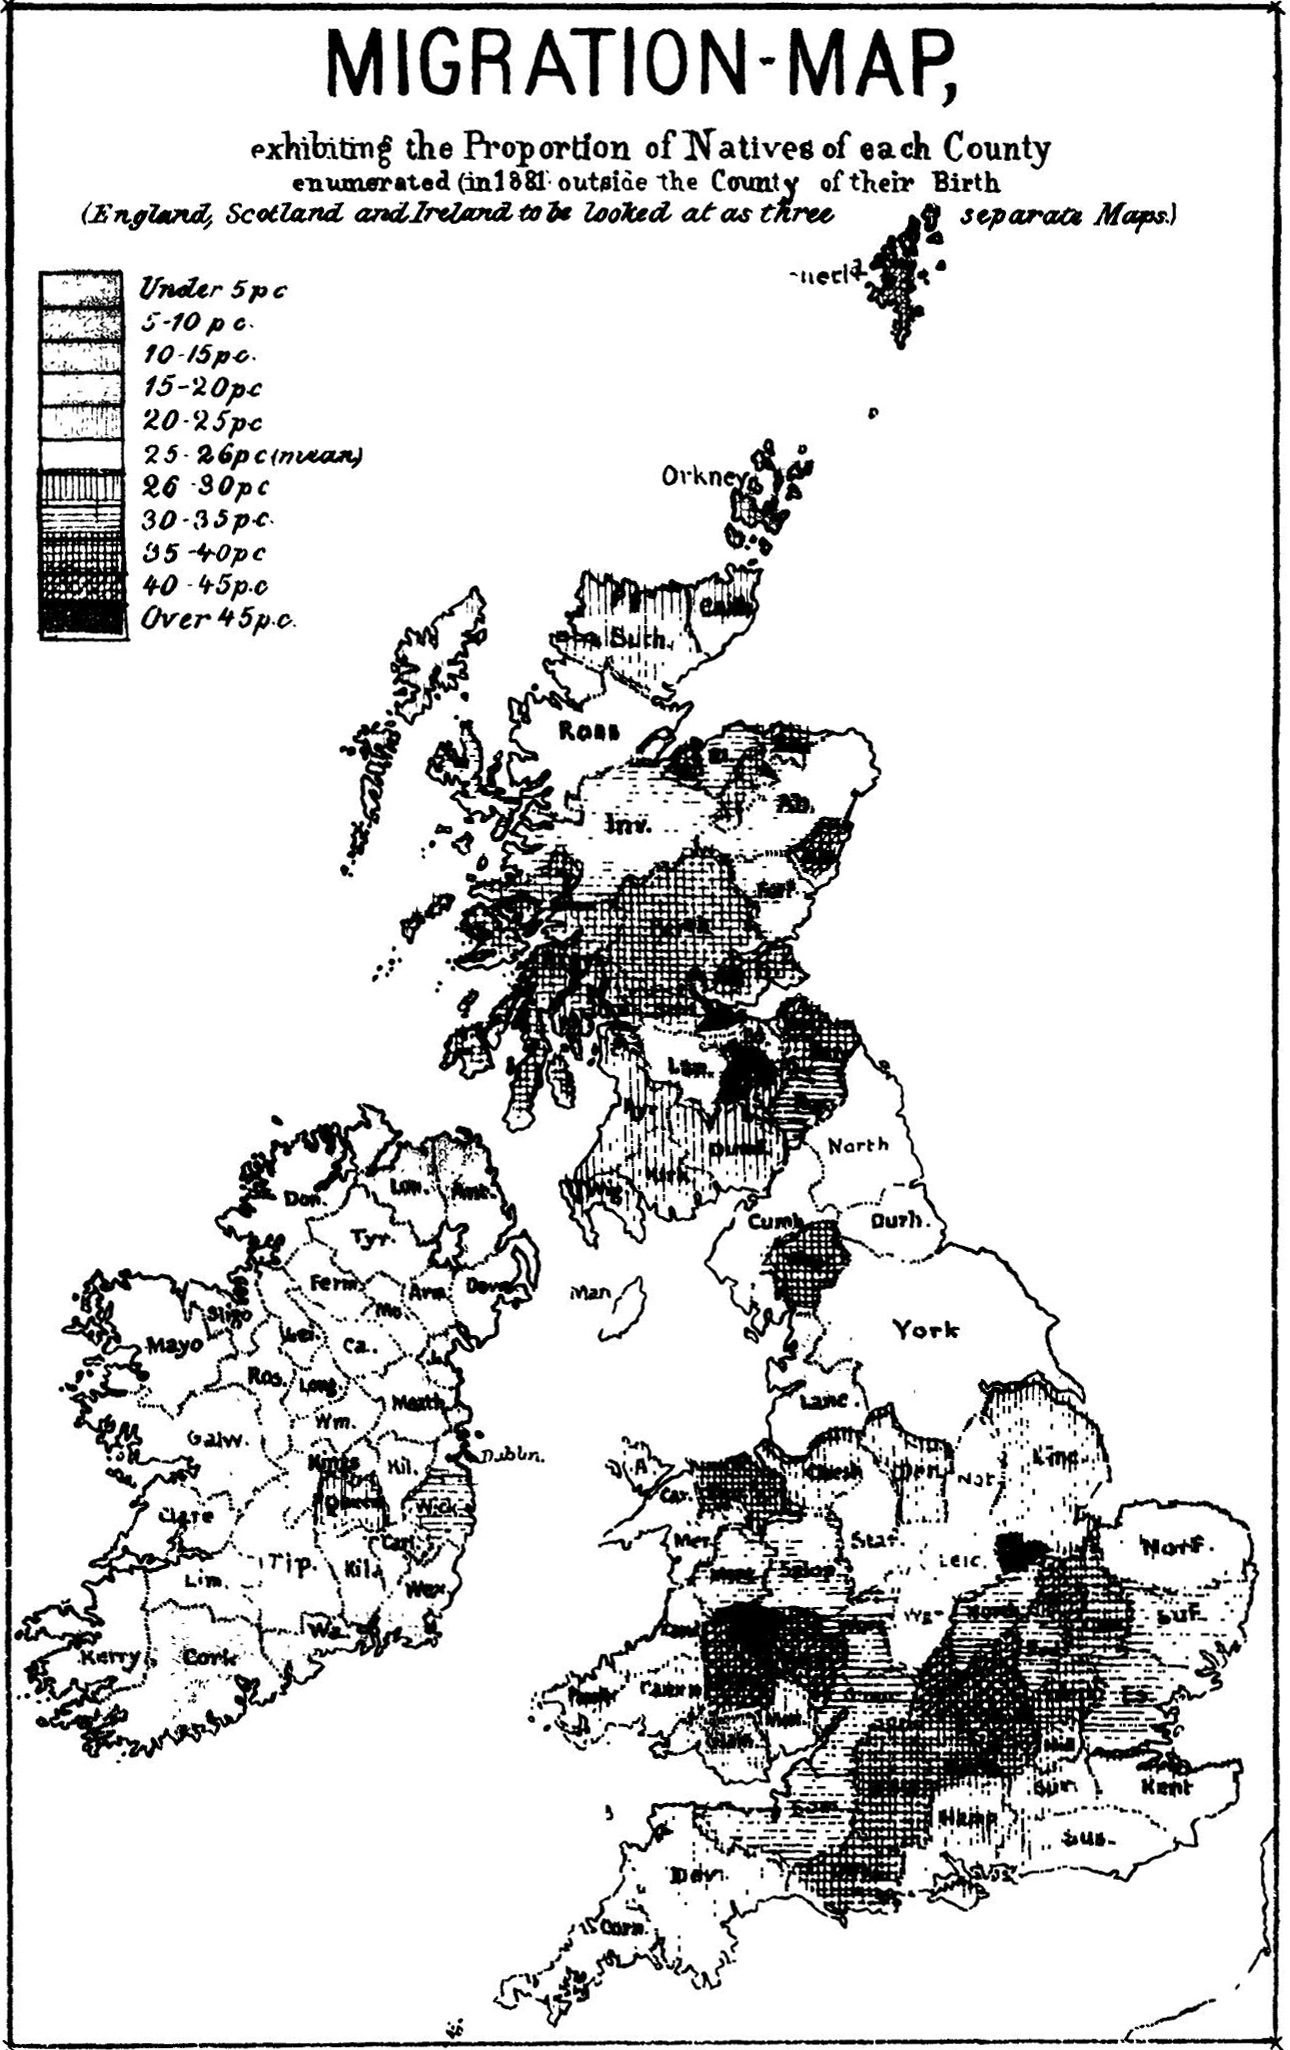
\includegraphics[width=0.28\textwidth]{britain.png}
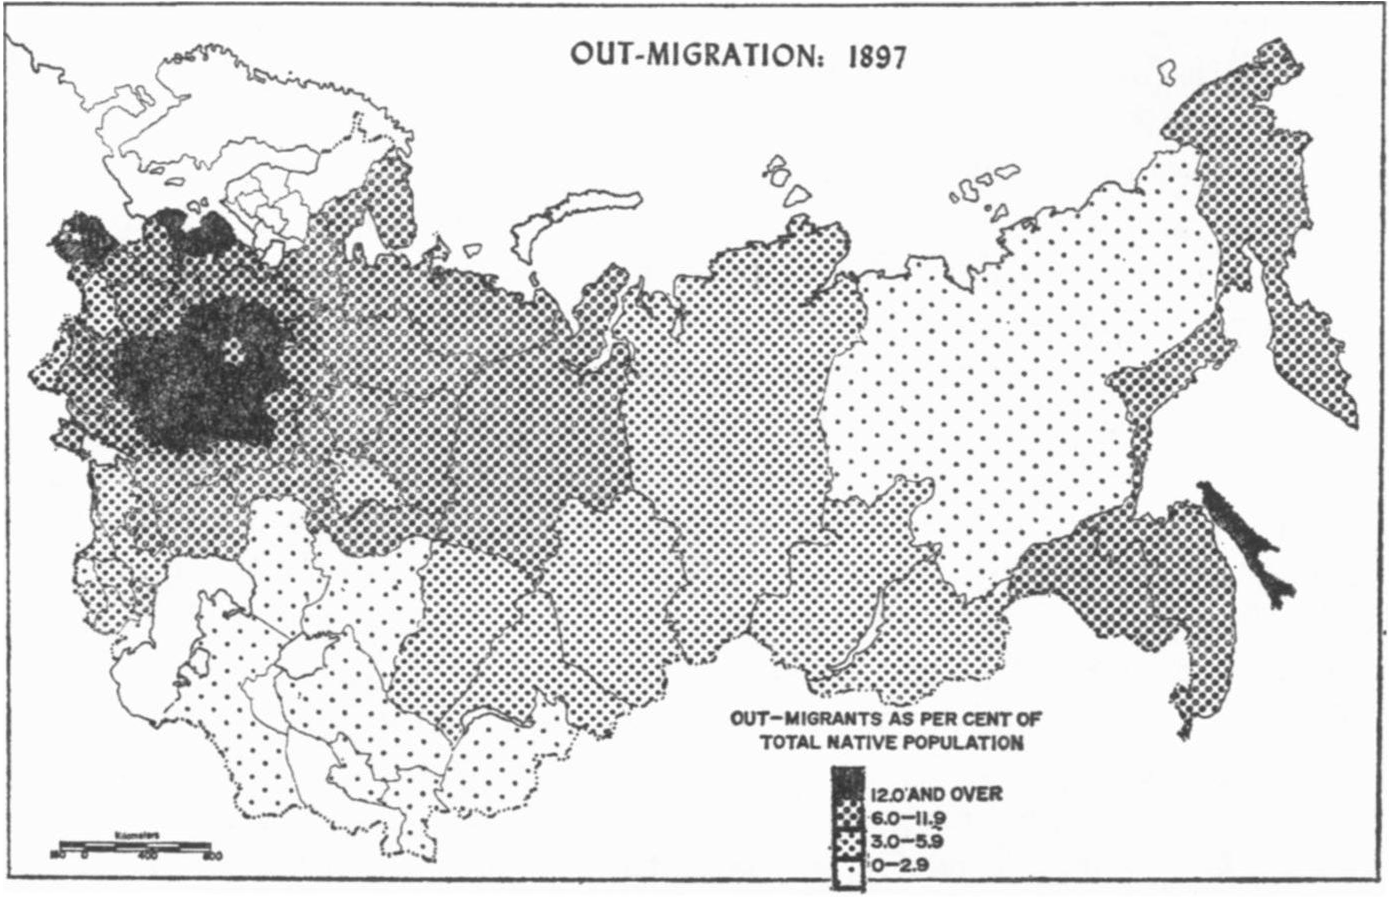
\includegraphics[width=0.68\textwidth]{russia.png}

\cite{ravenstein_laws_1885}; \cite{leasure_internal_1968}

\end{frame}

%\section{Российская империя в 19 веке}
\begin{frame}{Российская империя в 19 веке}
pics here
\end{frame}

%\section{Исследовательский вопрос}
\begin{frame}{Исследовательский вопрос}

Какие характеристики регионов влияли на внутренние миграции в Российской империи конца 19 века?
\par
Я анализирую влияние:
\begin{itemize}
	\item плотности населения и урбанизации
	\item социального развития (грамотности, естественного прироста населения)
	\item индустриального выпуска на душу населения
\end{itemize}

\end{frame}

{
\usebackgroundtemplate{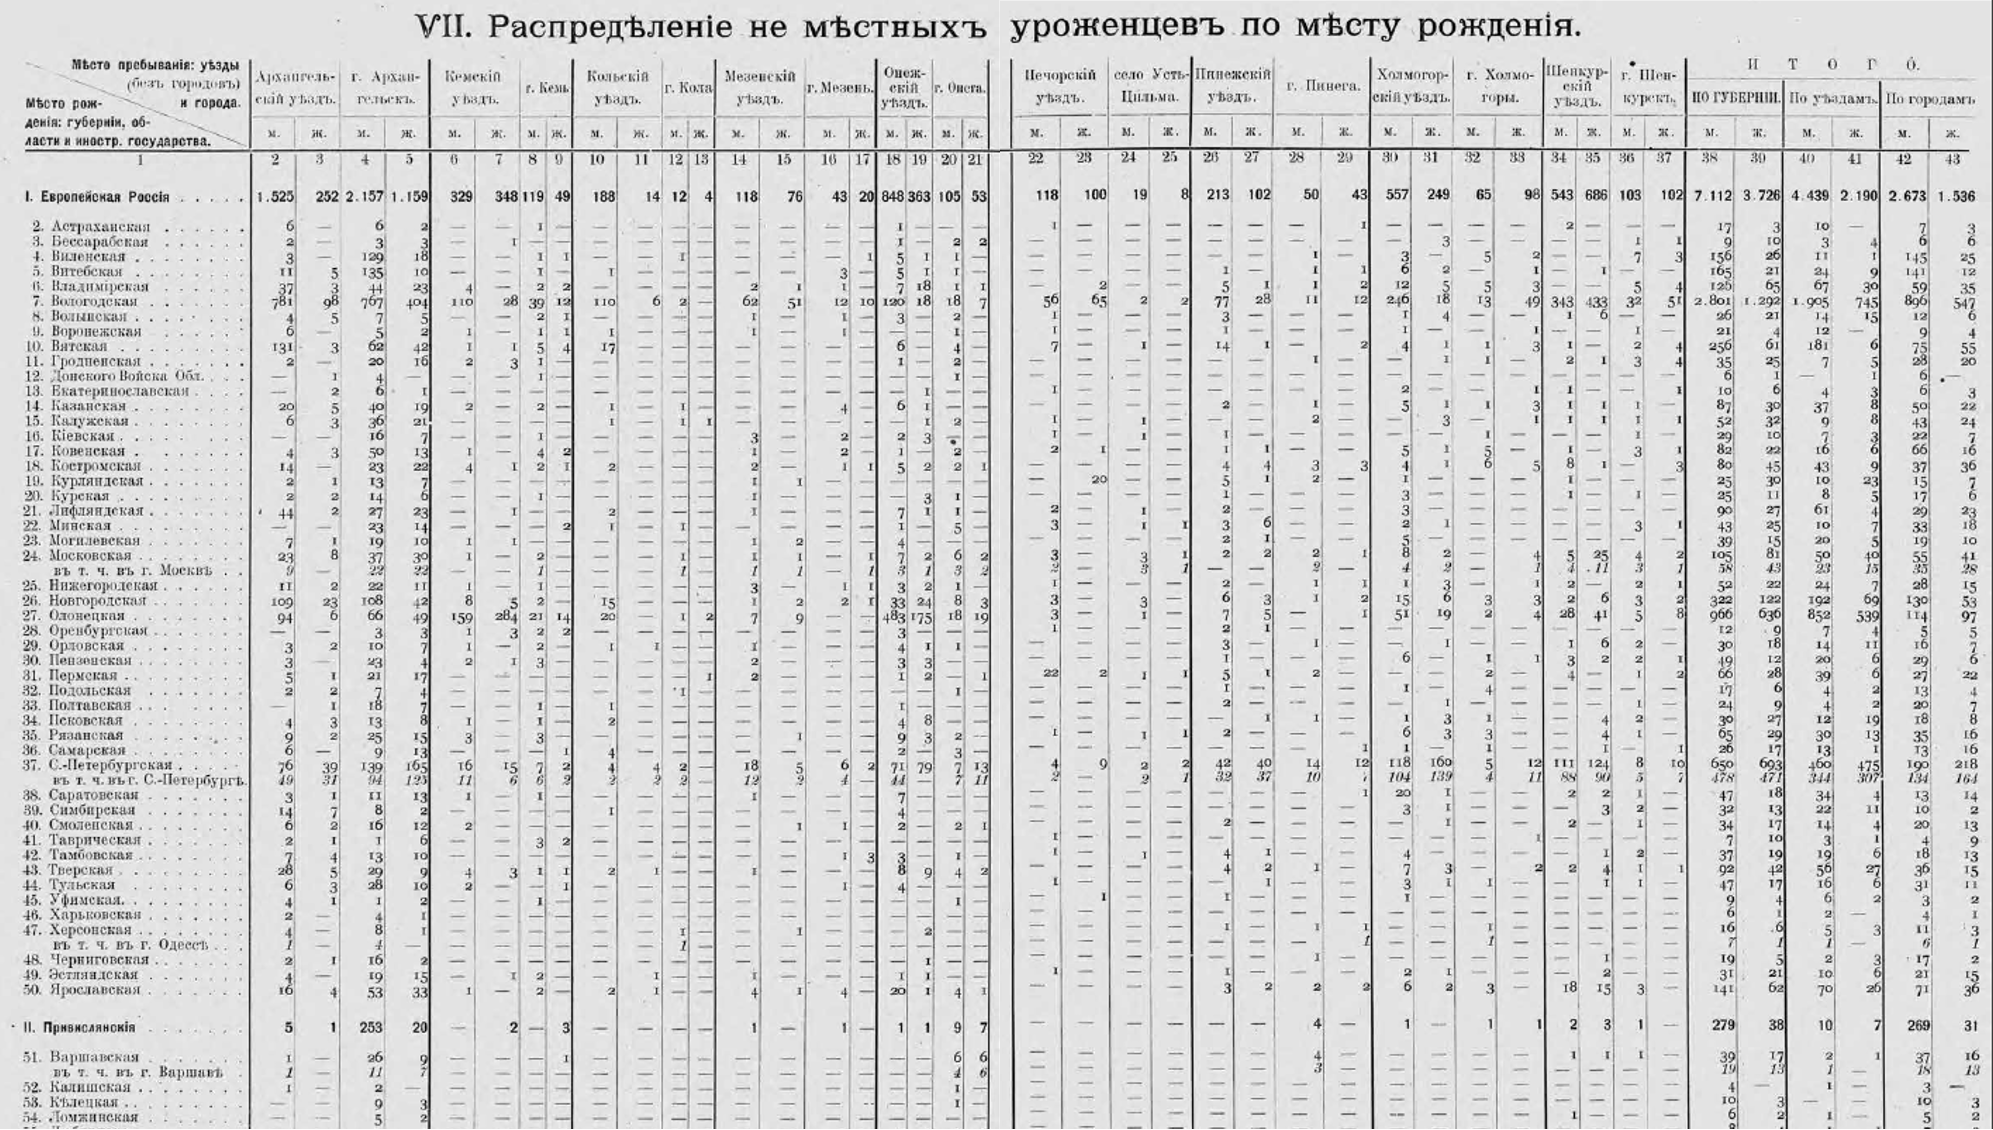
\includegraphics[width=\paperwidth]{census.png}}
\setbeamertemplate{navigation symbols}{}
\begin{frame}[b]
\hfill \colorbox{white}{\parbox{0.62\textwidth}{Первая всеобщая перепись населения \par Российской империи 1897 года \citep{census_1897}}}
\bigskip
\end{frame}
}

\section{Недостатки данных}
\begin{frame}{Недостатки данных}

\begin{itemize}
	\item Один год, кросс-секция
	\item Пожизненная миграция
	\item Нет важных экономических показателей и прочих переменных
\end{itemize}
\par
Ограниченная возможность делать каузальные выводы

\end{frame}

\begin{frame}{Миграция из регионов}
	
\begin{figure}[h!]
	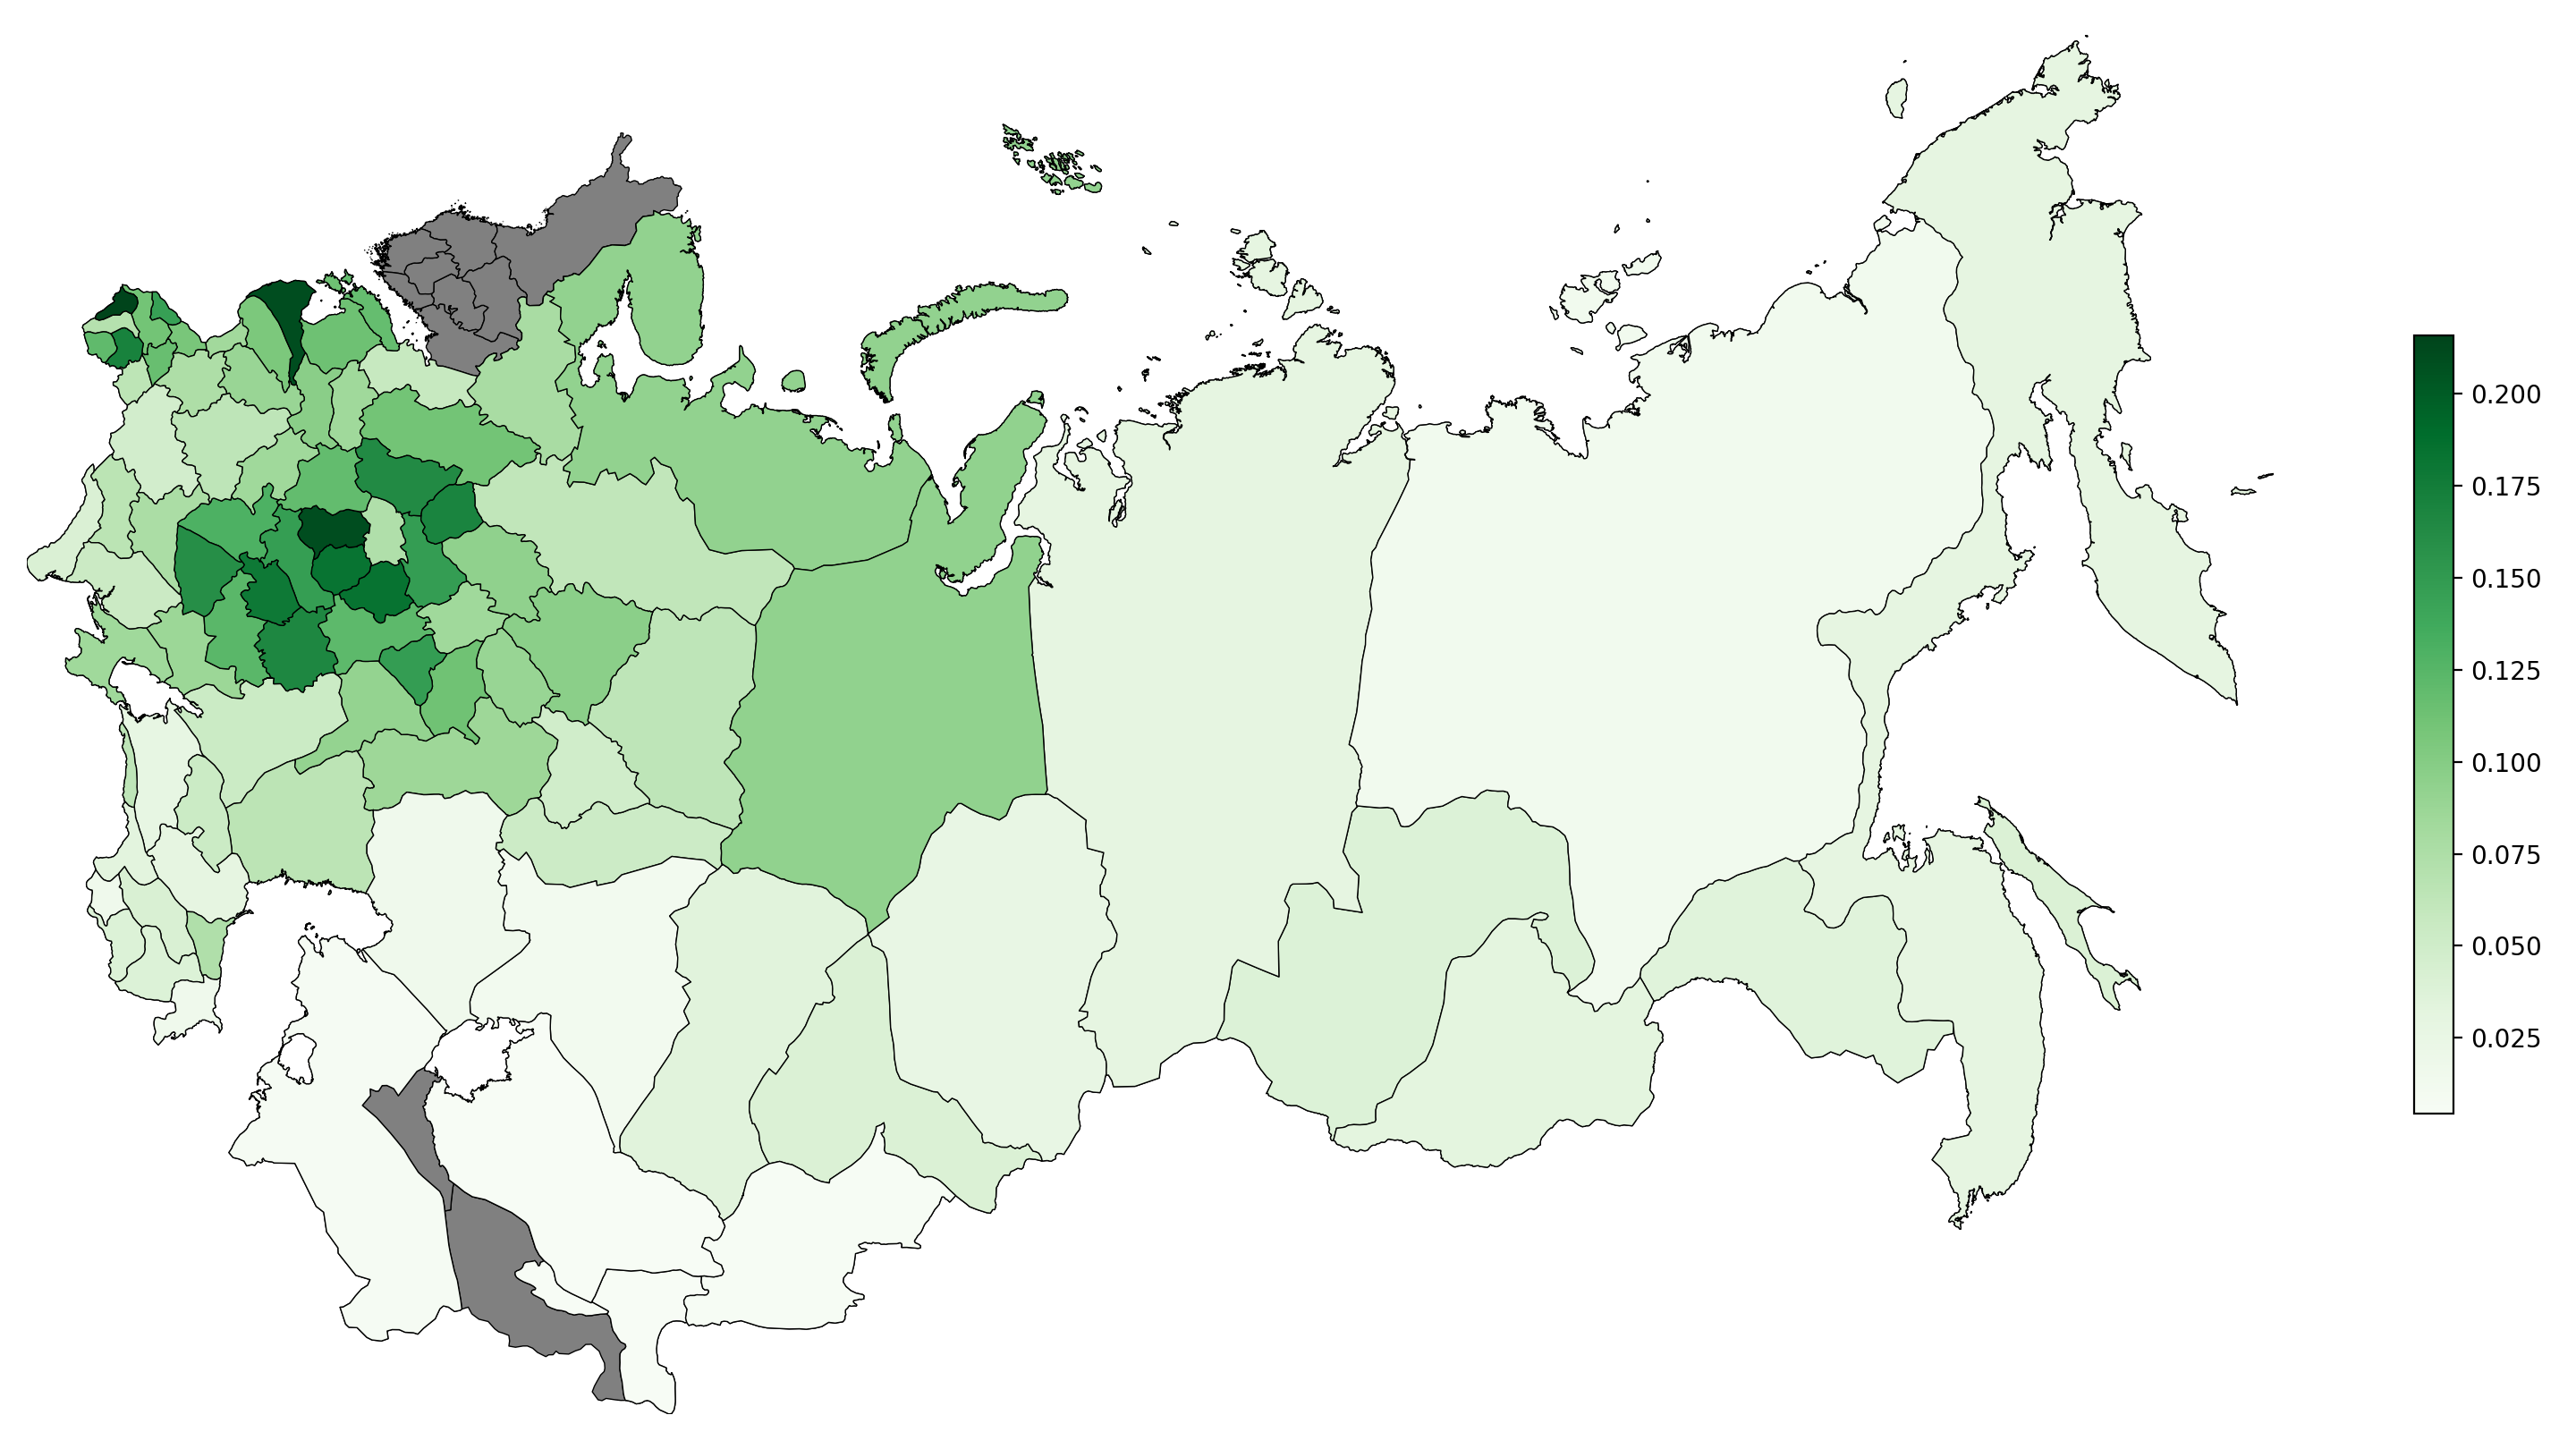
\includegraphics[height=0.8\textheight]{mig_of_pop_from.png}
\end{figure}
	
\end{frame}

\begin{frame}{Миграция в регионы}
	
\begin{figure}[h!]
	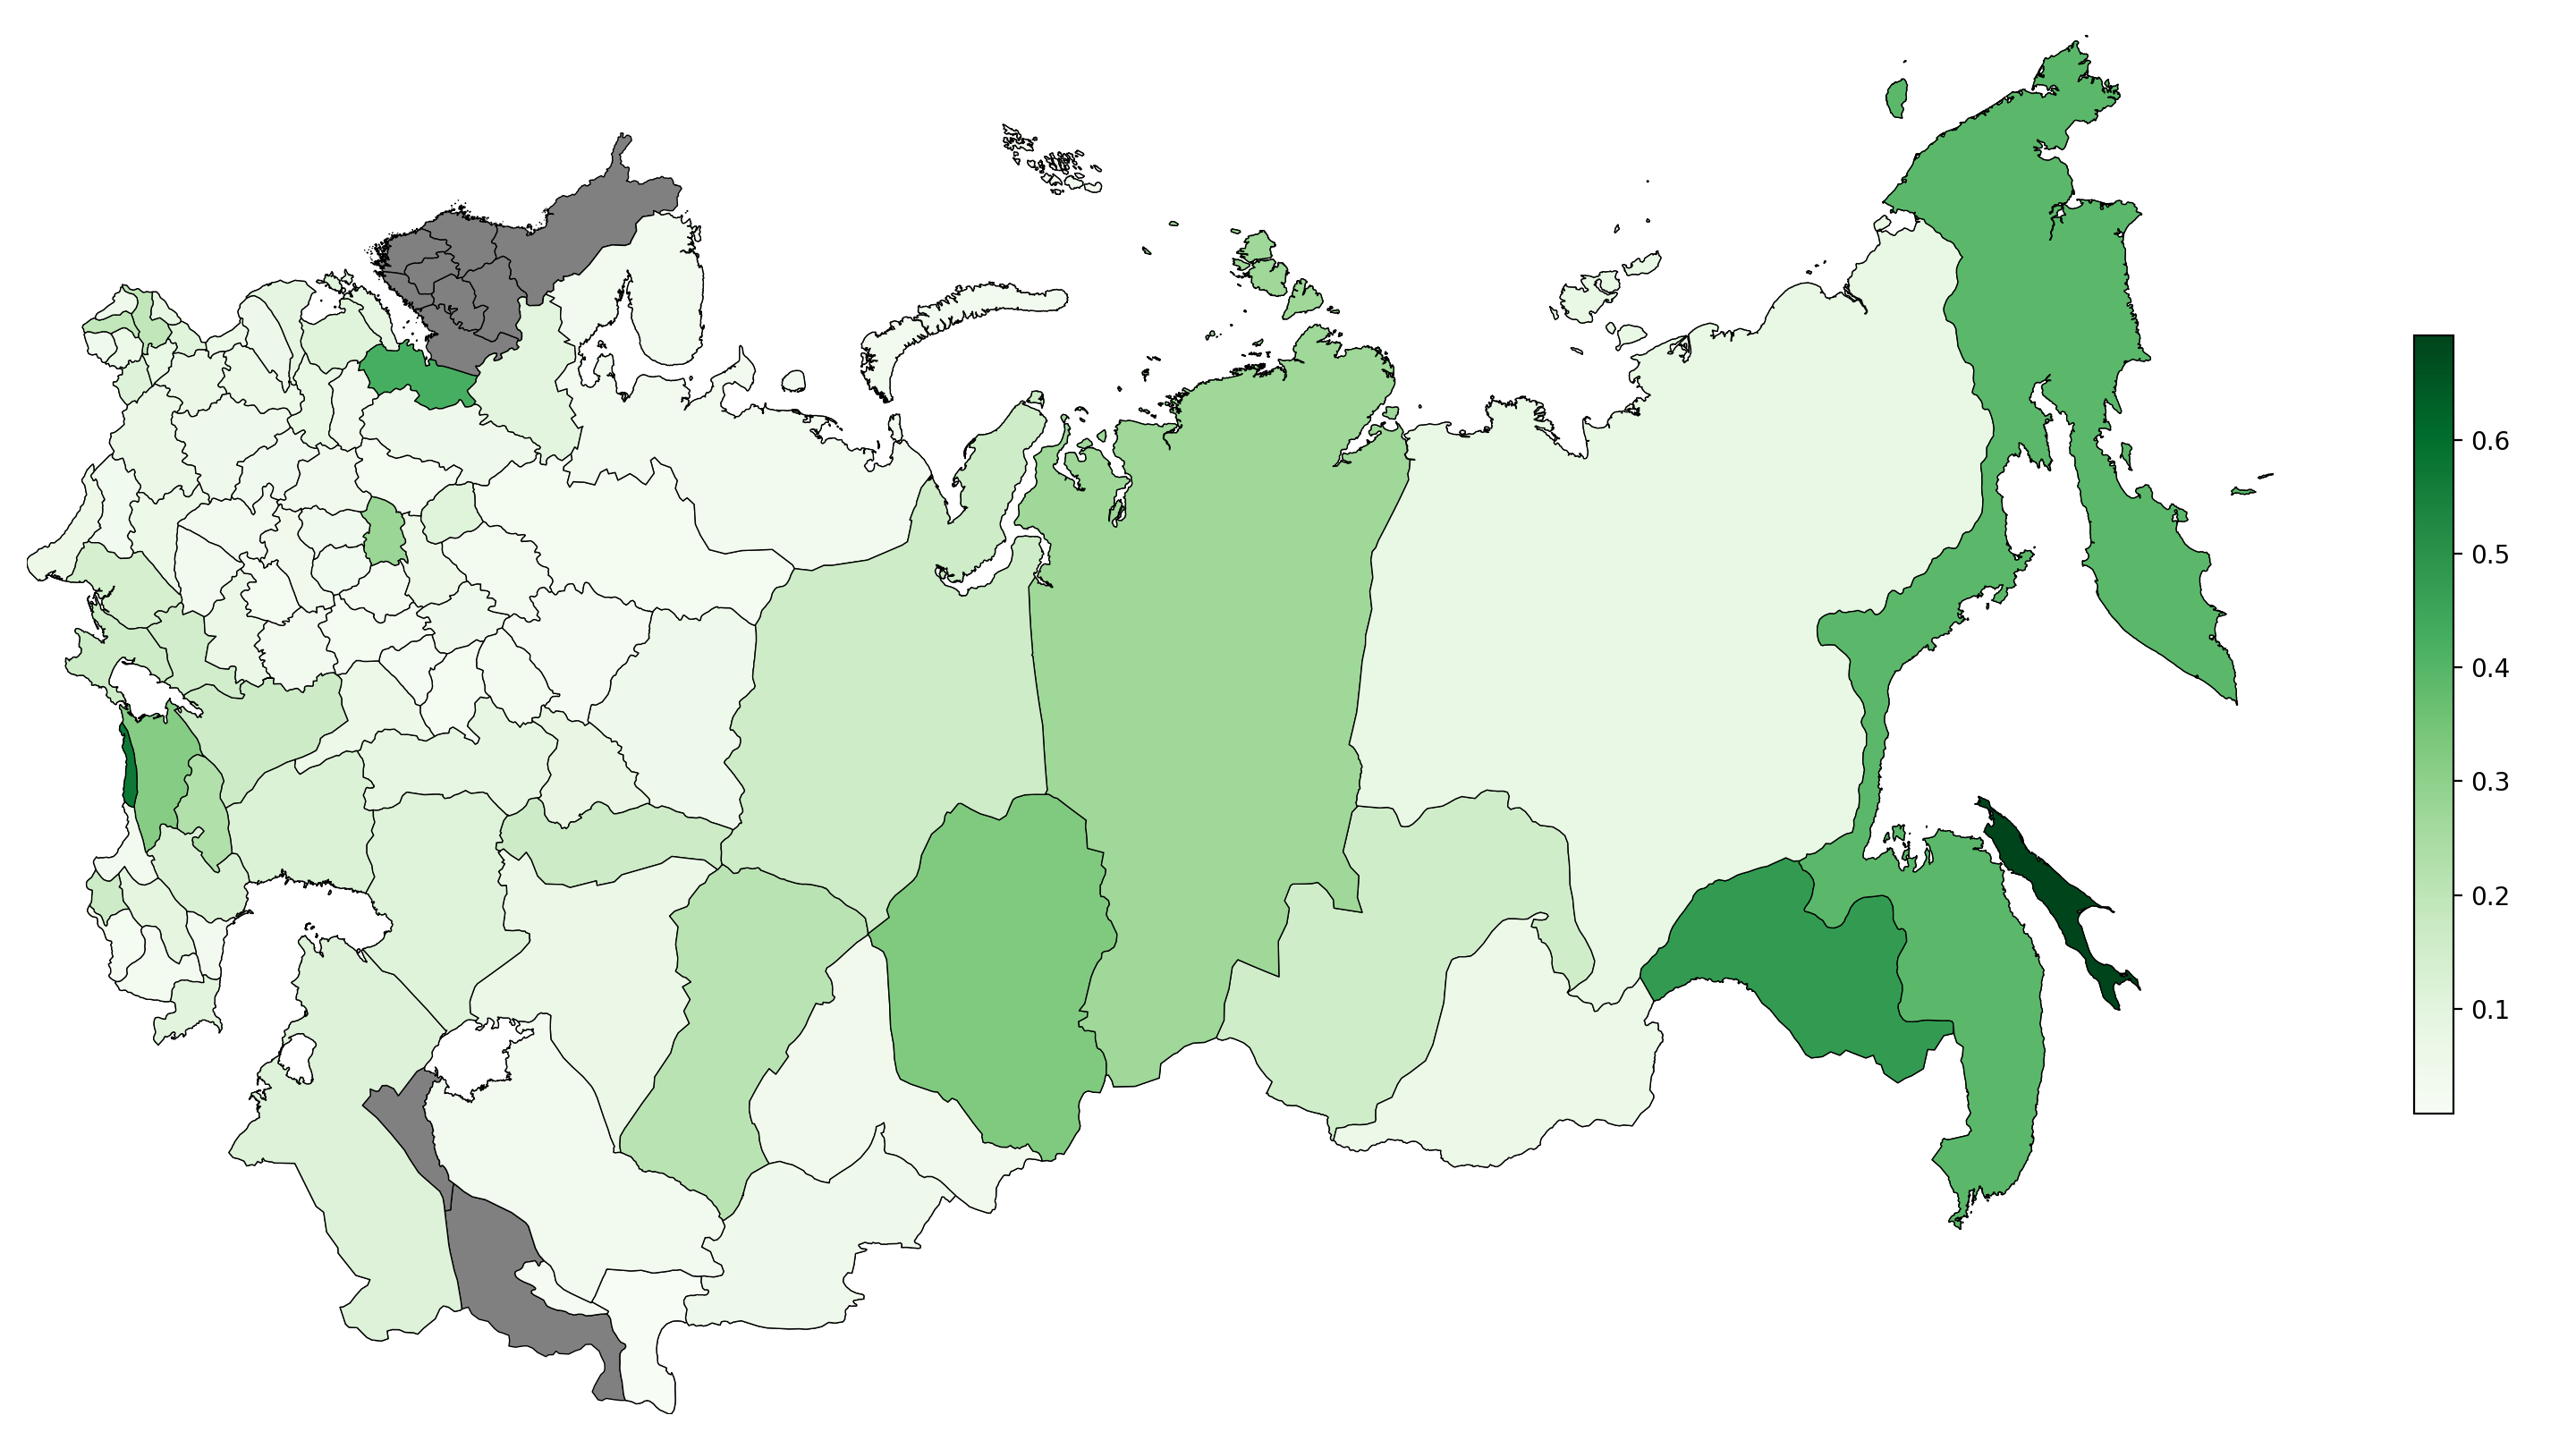
\includegraphics[height=0.8\textheight]{mig_of_pop_to.png}
\end{figure}
	
\end{frame}

\section{Гравитационная модель}
\begin{frame}{Гравитационная модель}

\begin{equation*}
	M_{ij} = \beta_0 P^{\beta_1}_{i} P^{\beta_2}_{j} D^{\beta_3}_{ij} + \varepsilon_{ij}
\end{equation*}

$M_{ij}$ – число переселенцев из региона $i$ в регион $j$; $P_i$ и $P_j$ -- население региона-источника и региона-назначения, $D$ -- расстояние, $\varepsilon$ -- случайный фактор.

PPML \citep{silva_log_2006}:
\begin{gather*}
	Pr[M_{ij}] = \frac{exp(-\mu_{ij})\mu^{M_{ij}}_{ij}}{M_{ij}!},\quad M_{ij} = (0, 1, ...) \\
	\mu_{ij} = exp(\beta_0 + S_i \beta_1^T + D_{j} \beta_2^T + X_{ij} \beta_3^T)
\end{gather*}

\end{frame}

\begin{frame}{Гипотезы}

\begin{columns}
	\begin{column}{0.60\textwidth}
		\begin{enumerate}
			\item На ранних этапах экономического развития, население концентрируется в крупных центрах
			\begin{equation*}
                    M_{ij} - M_{ji} = M_{ij} \left[ 1 - \frac{M_{ji}}{M_{ij}} \right] = M_{ij} \left[ 1 - \left( \frac{P_i}{P_j} \right)^{\beta_2 - \beta_1} \right]
			\end{equation*}
			Если $\beta_2>\beta_1$, $M_{ij}>M_{ij}$ \citep{poot_gravity_2016}
			\item Экономическое развитие (грамотность, выпуск промышленности) -- pull-факторы
			\item Перенаселение и низкая урбанизация -- push-факторы
		\end{enumerate}
	\end{column}
	
	\begin{column}{0.34\textwidth}
		\begin{table}
	\caption{Гипотезы}
	\label{table:hypo}
	\centering
	\begin{tabularx}{\textwidth}{XX}  %{@{}ll@{}}
		\toprule
		Переменная                   & Гипотеза                              \\ 
		\midrule
		$\textup{population}_i$, $\textup{population}_j$ & $\textup{population}_i < \textup{population}_j$ \\
		distance                     & $\approx-1$                            \\
		urbanization                 & $+$                                    \\
		density                      & $-$                                    \\
		literacy                     & $+$                                    \\
		industry                     & $+$                                    \\
		% $\Delta$climate              & $+$                                    \\
		% $\Delta$vars                 & $-$                                    \\ 
		\bottomrule
	\end{tabularx}
\end{table}
	\end{column}
\end{columns}

\end{frame}

% Commands to include a figure:
%\begin{figure}
%\includegraphics[width=\textwidth]{your-figure's-file-name}
%\caption{\label{fig:your-figure}Caption goes here.}
%\end{figure}

%\begin{table}
%\centering
%\begin{tabular}{l|r}
%Item & Quantity \\\hline
%Widgets & 42 \\
%Gadgets & 13
%\end{tabular}
%\caption{\label{tab:widgets}An example table.}
%\end{table}

\end{document}
